\documentclass[tikz,border=8pt]{standalone}
\usepackage{amsmath}
\usetikzlibrary{arrows.meta,positioning}

\begin{document}
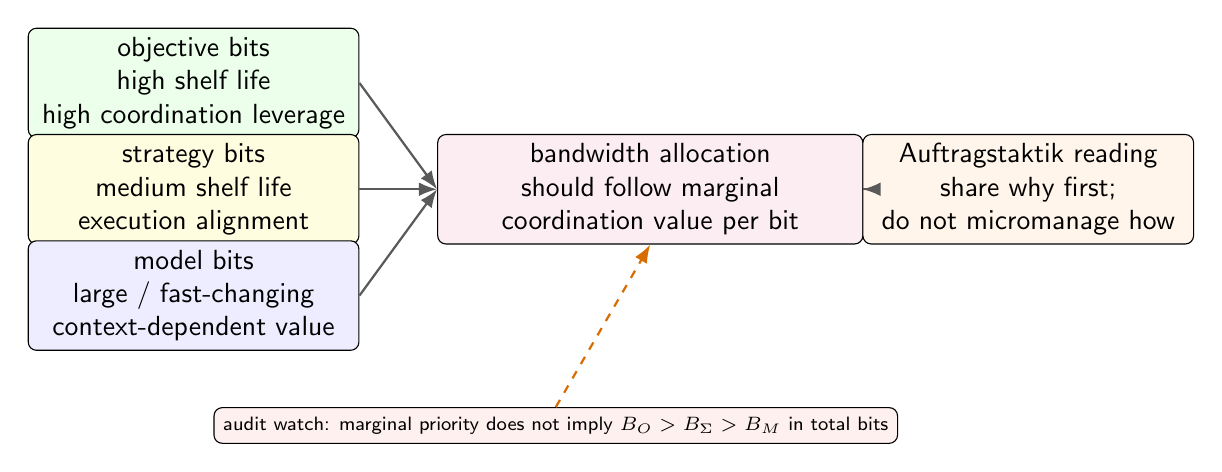
\begin{tikzpicture}[
  font=\sffamily,
  box/.style={draw, rounded corners=3pt, align=center, minimum width=42mm, minimum height=12mm, fill=white},
  note/.style={draw, rounded corners=3pt, align=center, font=\sffamily\scriptsize, fill=white},
  arrow/.style={-Latex, thick, draw=black!65},
  warn/.style={-Latex, thick, dashed, draw=orange!85!black}
]

\node[box, fill=green!8] (obj) at (-4.6,1.35)
  {objective bits\\high shelf life\\high coordination leverage};
\node[box, fill=yellow!12] (strat) at (-4.6,0)
  {strategy bits\\medium shelf life\\execution alignment};
\node[box, fill=blue!7] (model) at (-4.6,-1.35)
  {model bits\\large / fast-changing\\context-dependent value};

\node[box, fill=purple!7, minimum width=54mm] (alloc) at (1.2,0)
  {bandwidth allocation\\should follow marginal\\coordination value per bit};
\draw[arrow] (obj.east) -- (alloc.west);
\draw[arrow] (strat.east) -- (alloc.west);
\draw[arrow] (model.east) -- (alloc.west);

\node[box, fill=orange!8] (out) at (6.0,0)
  {Auftragstaktik reading\\share why first;\\do not micromanage how};
\draw[arrow] (alloc.east) -- (out.west);

\node[note, fill=red!6, minimum width=72mm] (audit) at (0,-3.0)
  {audit watch: marginal priority does not imply $B_O>B_\Sigma>B_M$ in total bits};
\draw[warn] (audit.north) -- (alloc.south);

\end{tikzpicture}
\end{document}
